\chapter{Appendix \autoref{chap:cvaml}}

\section{Implementation Details -- \autoref{sec:cvaml:empirical1}: Garnet}
\label{app:cvaml:model_design}

Each Garnet is defined by a randomly generated transition matrix and a random reward function.
Across all experiments we use 50 dimensional state spaces.
For each state $x_i$, we sample $k=10$ successor states at random without replacement.
Then we assign each successor state $x_j$ a weight $\omega_{ij} \sim \mathcal{N}(0, 1)$ and set the weight of all non-successor states to the floating point minimum.
The transition matrix is computed via the softmax function.
The reward is sampled as $r(x_i) \sim \mathcal{N}(0,1).$

This setup allows us to vary the stochasticity of the environment naturally.
The softmax temperature parameter $\tau$ controls the stochasticity.
As $\tau \rightarrow \infty$, the problem becomes deterministic with $p(x_j|x_i) = 1$ for the state $x_j$ with $\omega_{ij} = \argmax_j \omega_{i,j}.$
For $\tau \rightarrow \infty$, the probabilities for all successor states become equal $p(x_j|x_i) = \frac{1}{k}.$
In our experiments, we vary $\tau$ such that for almost all Garnets we obtain full determinism and equal transition probabilities, which empirically happens in the range $\tau \in [0.001, 10.0].$

\section{Implementation Details --  \autoref{sec:cvaml:empirical2}: DM Control}
\label{app:model_design}

\begin{table}[]
    \centering
    \begin{tabular}{l|c}
    Hyperparameter & Value \\\hline
    Batch size & 128\\
    Discount $\gamma$ & 0.99 \\
    Actor learning rate $\alpha_\pi$  & 0.0003 \\
    Critic learning rate $\alpha_Q$ & 0.0003 \\
    Model learning rate $\alpha_{\hat{p}}$  & 0.0003 \\
    Encoder learning rate $\alpha_\varphi$ & 0.0001 \\
    \end{tabular}
    \begin{tabular}{l|c}
     \\
    Model rollout depth $m$ & 1 \\
    Model bootstrap depth $b$ & Varied (0 and 1) \\
    Model samples $k$ & Varied (1 and 4) \\
    Proportion real $\rho$ & 0.9 \\
    Latent dimension & 512 \\
    Gradient clipping & 10 \\
    \end{tabular}
    \caption{Hyperparameter of the deep learning experiments. Aside from the $(m,b)$-(C)VAML relevant hyperparameters, we keep all others consistent across environments and algorithms.}
    \label{tab:cvaml:hyperparams}
\end{table}

\subsection{Architecture}
The original MuZero paper \parencite{schrittwieser2020mastering} provides large-scale experiments on the ALE benchmark \parencite{bellemare13arcade}.
However, the original algorithm and the ALE suite are computationally extremely expensive to run.
In addition, to the best of our knowledge, no reliable open-source replication of the closed-source MuZero and Stochastic MuZero models and algorithms exists.
Instead, we use the TD-MPC architecture and algorithm \parencite{hansen2022temporal} as our main reference.
This implementation uses the MuZero loss but is significantly cheaper and faster to run in a small-scale experimental setting, while still solving non-trivial control tasks.

We adopt the architecture and model-based MPC search procedure of \textcite{hansen2022temporal} as our baseline model.
In addition to the $L_2$ based deterministic latent setup, we also use a Gaussian latent model as our stochastic environment model.
This implementation follows similar ideas used in observation-space models, such as \textcite{pets,mbpo}.
While the stochastic environment models used in Dreamer \parencite{hafner2021mastering} would have been an alternative, it has not shown strong performance in continuous control tasks and is significantly more expensive to run.
In addition, \textcite{voelcker2024when} shows that observation-space reconstruction can be a suboptimal auxiliary task for aligning a latent space with value function prediction.
Finally, we adopt the joint model-free and model-based training proposed in \textcite{voelcker2025mad}.
For the MuZero setting ($b=1$) we update the value function both for the state and the predicted latent state.
In the IterVAML setting, there is no meaningful way to update the model's predicted value function, and therefore we only update the current state's value function.

Code is provided in the supplementary files and open-sourced after the review process.

Hyperparameters can be found in \autoref{tab:cvaml:hyperparams}.

\subsection{Environment}
\label{app:stoch_env}
As several recent papers have shown, the vast majority of environments in the DM Control suite are effectively saturated. 
We, therefore, restrict our experiments to the most difficult domains, \emph{humanoid} and \emph{dog}, on which large performance differences still appear \parencite{nauman2024bigger,voelcker2025mad,fujimoto2025towards}.


\subsection{Additional results}

In addition to the raw performance graphs in the main paper, we present the average model entropy and VAML loss curves in \autoref{fig:vaml_entropy}.
As expected, we find that the CVAMl loss leads to a higher entropy model compared to the VAML loss.
This however does not lead to a noticeable difference in the VAML error itself.

\begin{figure}[h]
    \centering
    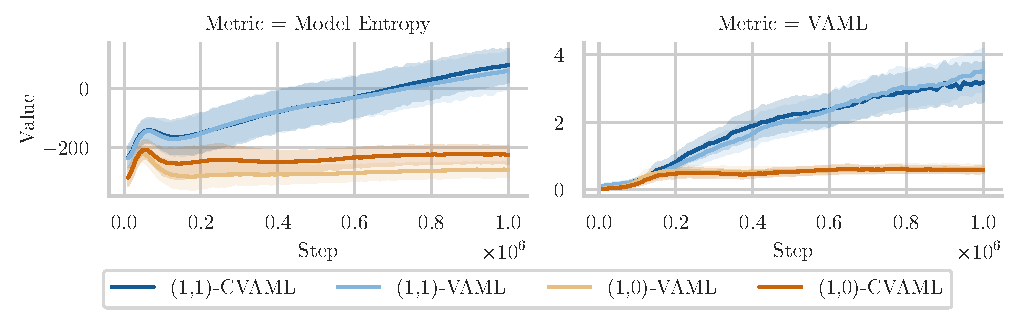
\includegraphics[width=0.9\textwidth]{figures/lambda/plts/app_metrics.pdf} 
    \caption{Model entropy (left) and loss value for the VAML-losses (right) aggregated across all environments. The shaded area represents a 95\% stratified bootstrap interval. We see that the model entropy of the corrected $(1,0)$-VAML differs significantly, as we expect. However, this does not translate to a pronounced difference in the VAML error itself. Therefore, while the calibration term does indeed lead to a higher variance, this does not directly translate into an improvement in performance. In $(1,1)$-VAML, the model entropy does not differ significantly, however, without calibration, the VAML error seems to be growing slightly stronger (although not outside of overlapping confidence intervals). Given the large deviation in performance we observe in the main results for $(1,1)$-VAML, we conjecture that correcting the value function learning term is significantly more important for performance.}
   \label{fig:vaml_entropy}
\end{figure}
